\section{Camera}
\label{sec:c270}

The camera used in this project is the C270 HD WEBCAM, shown in \cref{fig:camera}, a USB 2.0 webcam manufactured by Logitech. It features a CMOS sensor capable of capturing video at a resolution of 640 x 480 pixels at 30 frames per second. Its compact design and USB interface allow for easy integration into the experimental setup for real-time image acquisition and processing of the interferometer fringes pattern.

This camera was selected due to its balance between cost and performance, while it may not offer high speed or high-resolution capabilities, it is sufficient for the requirements of this project in a calibration stage. The camera's output is processed by a common python library used for computer vision tasks, OpenCV.

\begin{figure}[htbp]
    \centering
    \begin{subfigure}{0.45\textwidth}
        \centering
        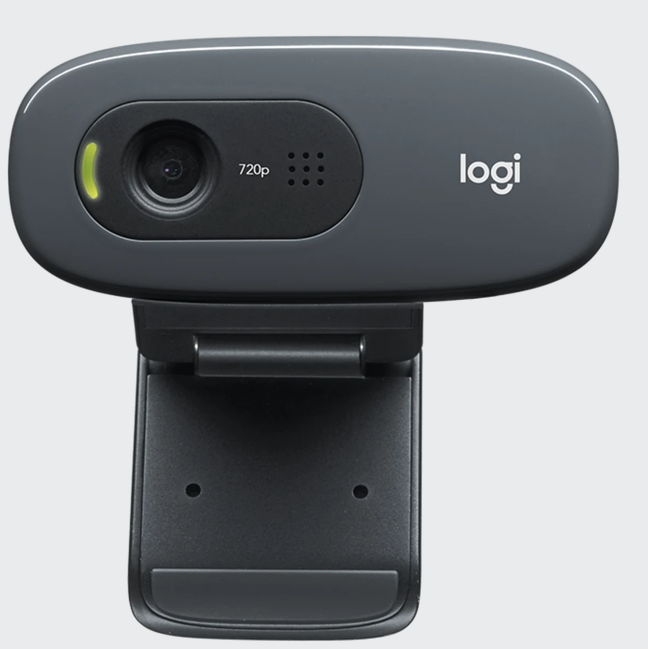
\includegraphics[width=\textwidth]{images/camera.png}
        \caption{C270 HD WEBCAM}
        \label{fig:camera}
    \end{subfigure}\hfill
    \begin{subfigure}{0.45\textwidth}
        \centering
        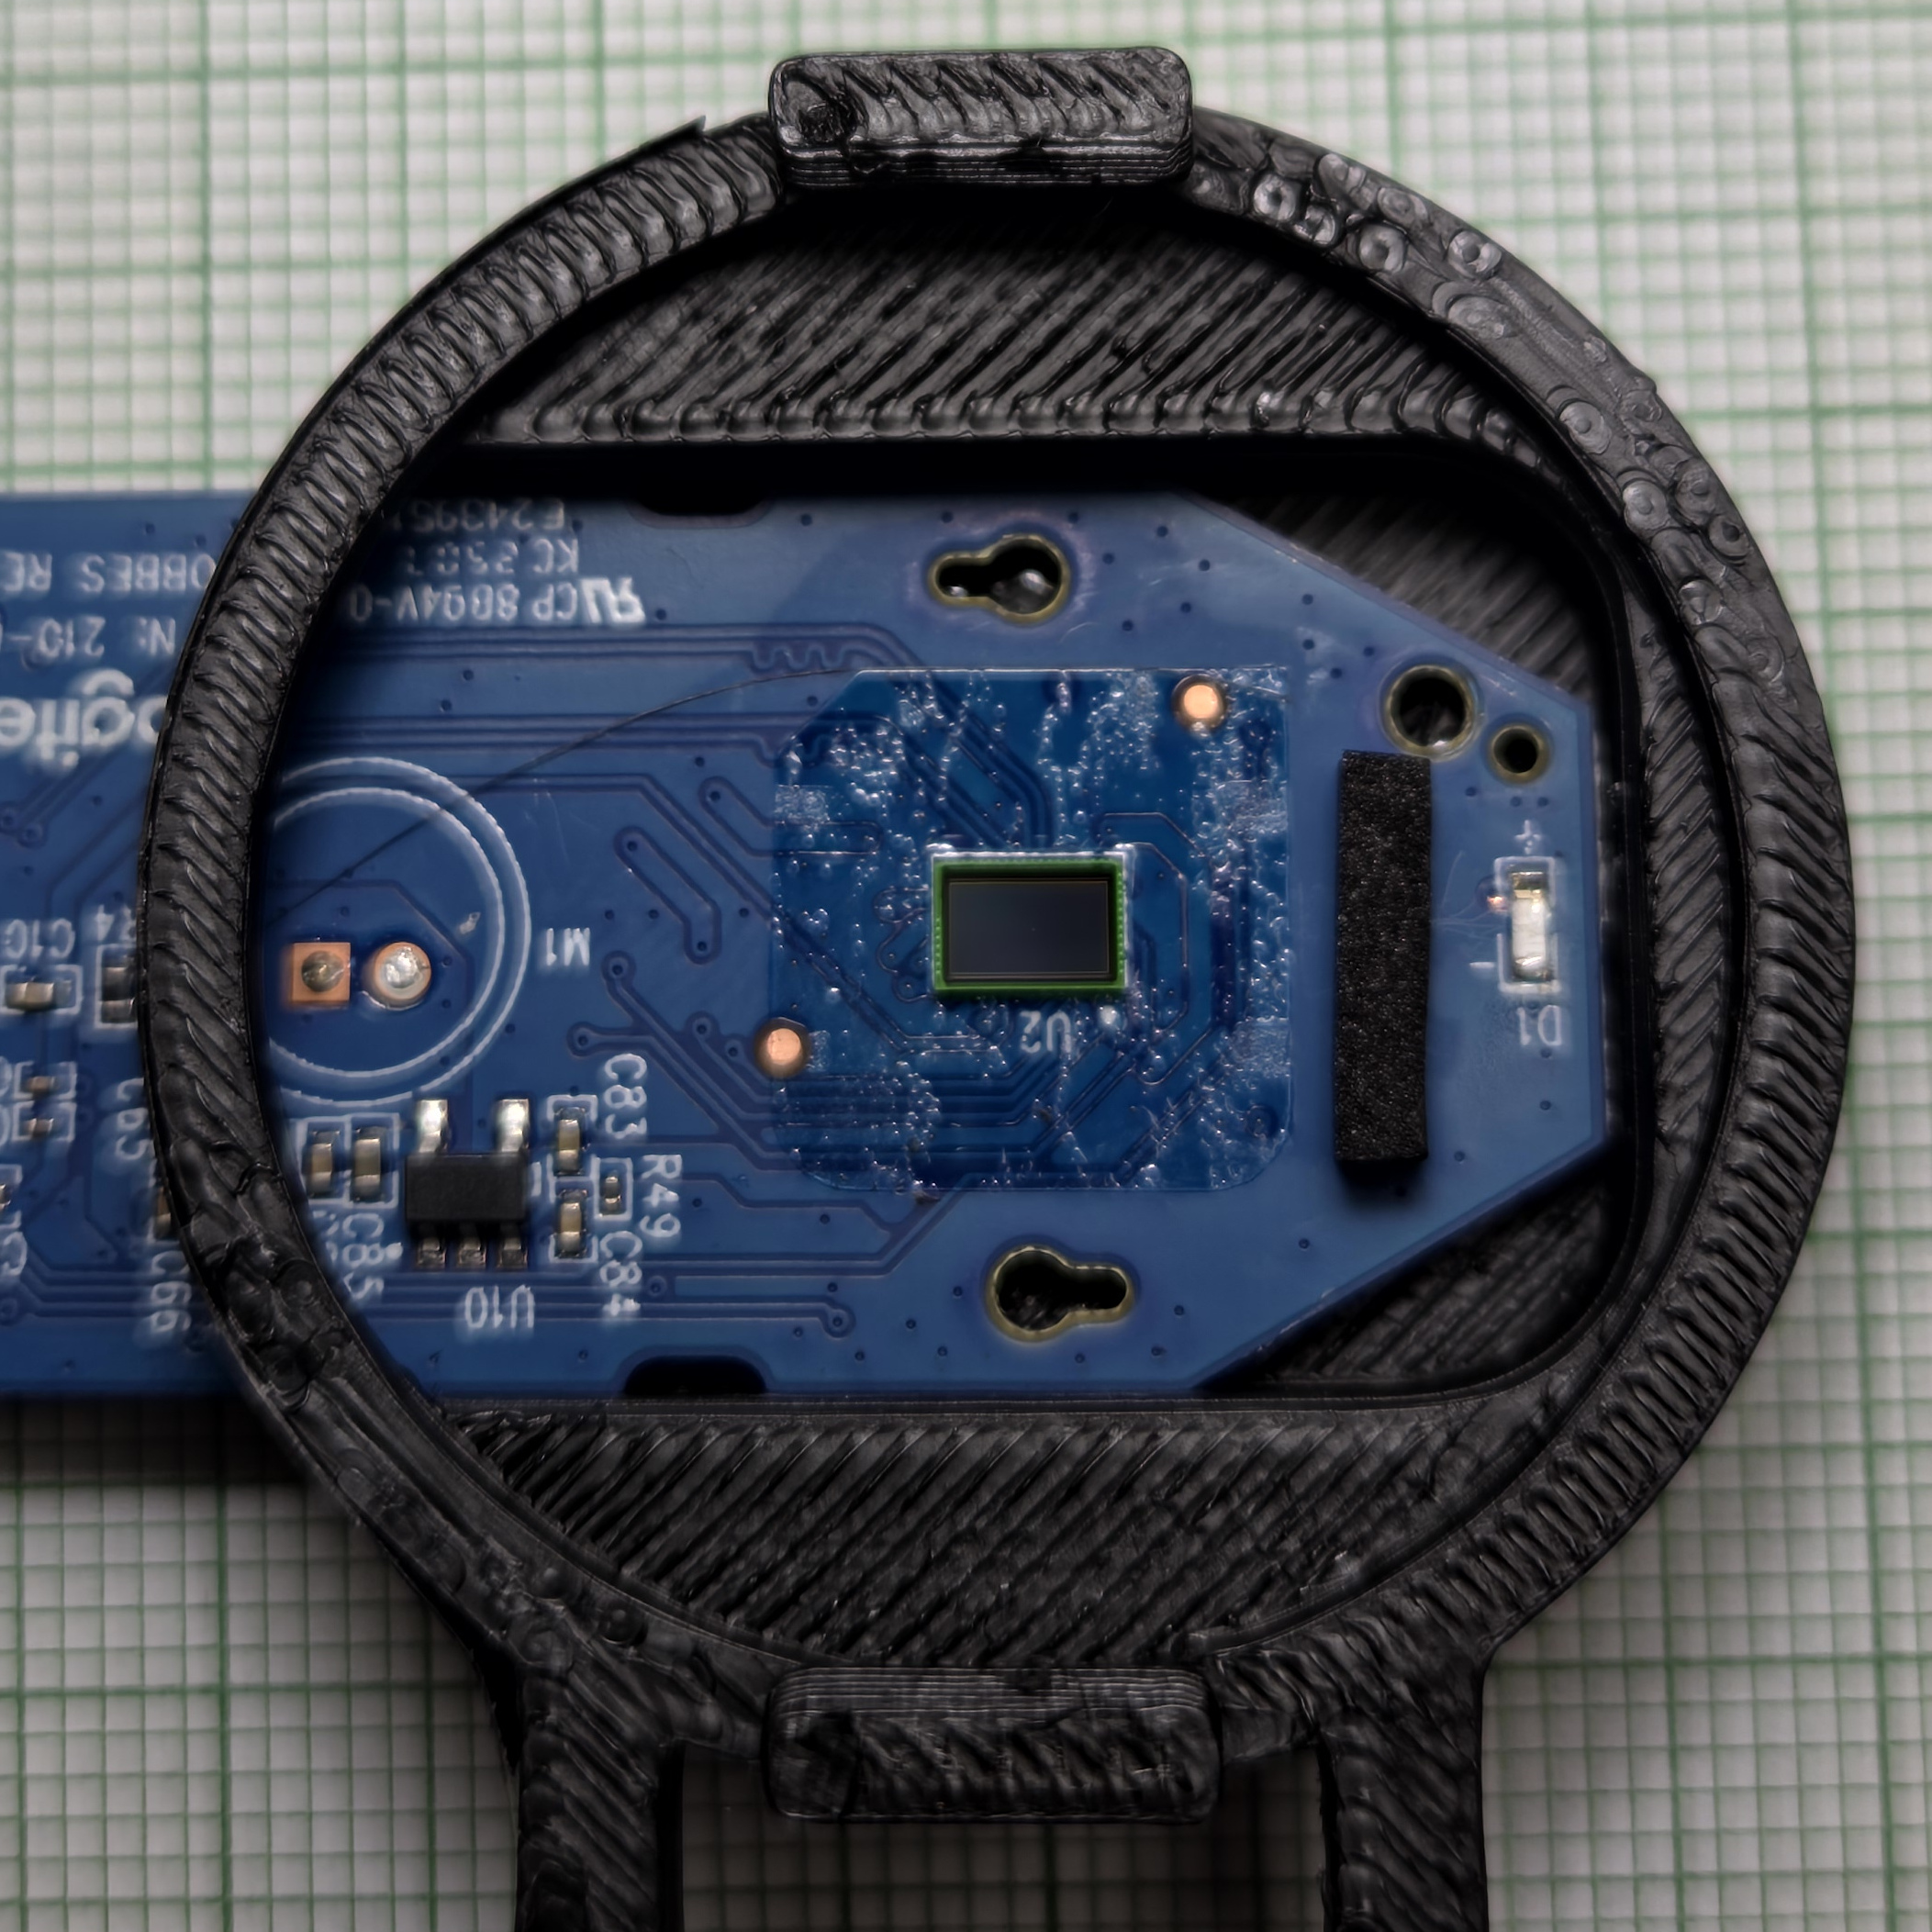
\includegraphics[width=\textwidth]{images/c270_on_holder.jpg}
        \caption{Camera Sensor with 3D Printed Support}
        \label{fig:camera_exposed}
    \end{subfigure}
    \caption{Camera Experimental Setup. a) C270 HD WEBCAM; b) Camera Sensor with 3D Printed Support for coupling to the interferometer setup.}
    \label{fig:camera_setup}
\end{figure}

The camera is dismantled to access the sensor directly, allowing for a more compact and flexible integration into the experimental setup, the lens was removed to avoid distortion of the pattern \cref{fig:camera_exposed}. A 3d printed support was designed to hold the camera in place, ensuring stability and proper alignment with the interferometer's optical path. The camera is connected to a computer via USB, where the acquired images are processed in real-time to extract the fringes and count their movement. This support belongs to a modular set of 3D-printed mounts, described in \cref{sec:experimental_setup}.


\subsection{Acquisition Graphical User Interface}
\label{sec:camera_gui}

To apply the ROI-based fringe tracking described in \cref{sec:roi_fringe_velocity} to the frames delivered by the C270 camera (\cref{sec:c270}), a custom graphical user interface (GUI) was developed. It gathers in a single window the live camera view, the placement and adjustment of the $\text{ROI}$, the real-time plot of the mean ROI irradiance, and the control of the stepper motor that drives the movable mirror, so that an experiment can be configured, executed and monitored without leaving the application. The interface is shown in \cref{fig:camera_ui}.

\begin{figure}[htbp]
    \centering
    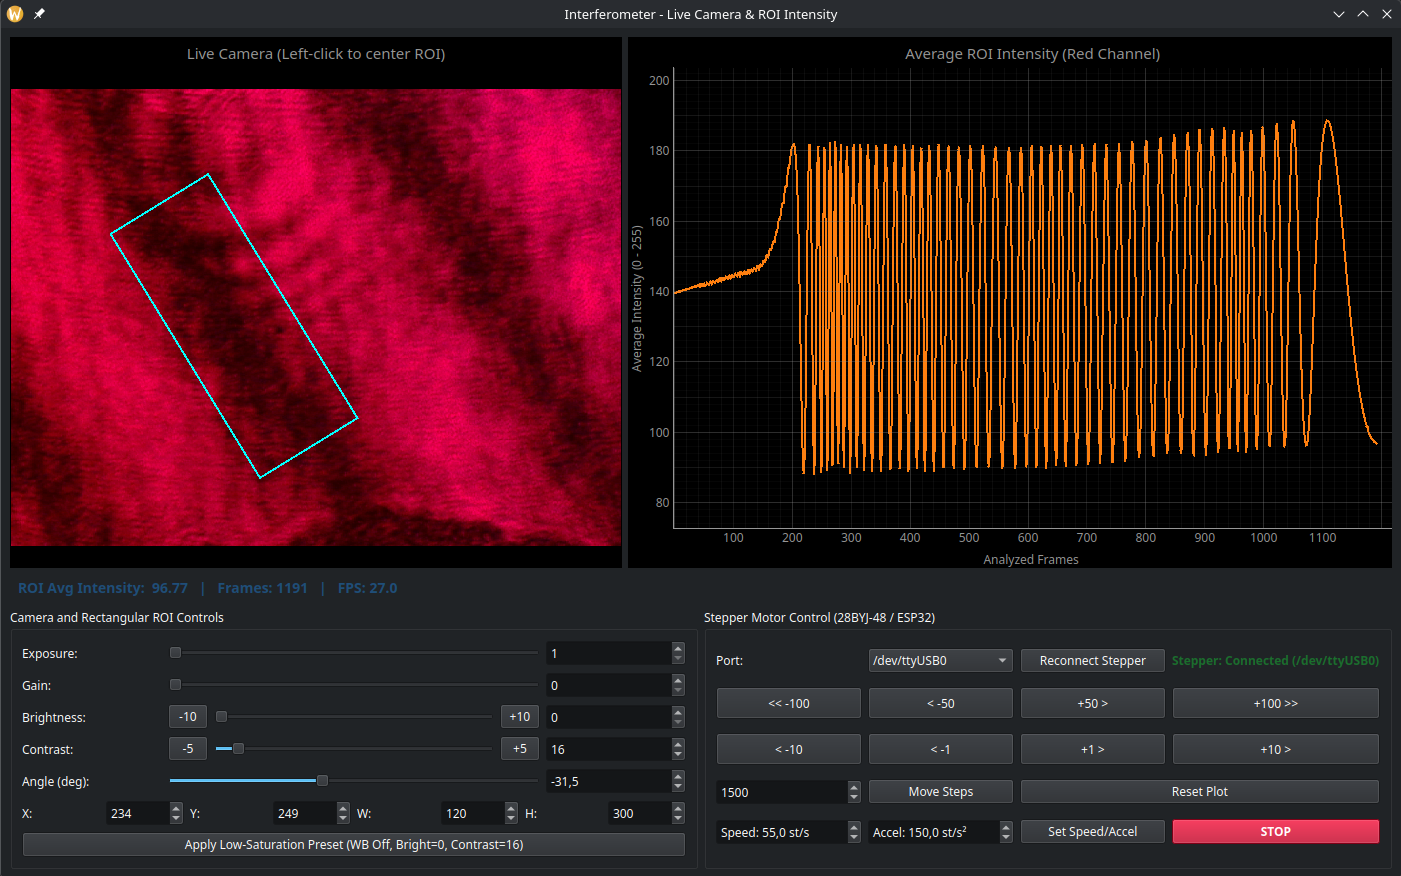
\includegraphics[width=\textwidth]{images/camera_ui.png}
    \caption{Graphical user interface for live fringe acquisition. Top left: live camera view with the rotated rectangular $\text{ROI}$ (cyan); top right: average $\text{ROI}$ intensity of the red channel versus analyzed frames; middle: status line with ROI average intensity, frame counter and FPS; bottom left: camera and $\text{ROI}$ controls; bottom right: stepper motor control.}
    \label{fig:camera_ui}
\end{figure}

The window is divided into the following regions:
\begin{itemize}
    \item \textbf{Live camera view:} Displays the frames captured by the camera in real time. The $\text{ROI}$ is drawn over the image as a cyan rectangle and can be re-centered at any moment with a left click on the desired position. The $\text{ROI}$ can be rotated by an angle (in degrees), allowing its long side to be aligned with the local fringe direction and its width $W$ to be matched to the fringe period $\Lambda_x$, which controls the attenuation of the modulation amplitude in \cref{eq:roi_sinc_attenuation}.

    \item \textbf{ROI intensity plot:} For every analyzed frame $k$, the mean irradiance $\bar{I}_{\text{ROI}}(t_k)$ of the red channel inside the $\text{ROI}$ \cref{eq:roi_mean_irradiance} is appended to a live plot, with intensity in the $0$--$255$ range on the vertical axis and the number of analyzed frames on the horizontal axis. Each oscillation of the trace corresponds to a fringe crossing the $\text{ROI}$, so the maxima and minima used to count fringes and compute the mirror displacement \cref{eq:roi_step_displacement} can be inspected visually.

    \item \textbf{Status line:} Reports the current ROI average intensity, the number of frames processed and the effective frame rate (FPS). The latter is relevant because the maximum measurable velocity is limited by the sampling rate (see \cref{sec:camera_velocity}); in the example the camera runs at $27.0$ FPS, slightly below the nominal $30$ FPS.

    \item \textbf{Camera and ROI controls:} Sliders and numeric fields set the exposure, gain, brightness and contrast of the camera, together with the $\text{ROI}$ geometry ($X$, $Y$, $W$, $H$ and angle). A \emph{low-saturation preset} button disables the automatic white balance and sets brightness to $0$ and contrast to $16$. Avoiding pixel saturation is important because a clipped signal flattens the peaks of $\bar{I}_{\text{ROI}}(t_k)$ and degrades the detection of maxima and minima.

    \item \textbf{Stepper motor control:} Communicates over a serial port with the ESP32 that drives the 28BYJ-48 stepper motor. The panel allows selecting the port and reconnecting, moving a relative number of steps with the quick buttons ($\pm 1$, $\pm 10$, $\pm 50$, $\pm 100$) or an arbitrary count with \emph{Move Steps}, setting the cruise speed (steps/s) and acceleration (steps/s$^2$), clearing the plot with \emph{Reset Plot} before a new measurement, and stopping the motor immediately with the \emph{STOP} button.
\end{itemize}

During the Openflexure calibration, the operator positions and orients the $\text{ROI}$, applies the low-saturation preset, resets the plot and commands a known number of motor steps. The fringes counted in the resulting trace, together with \cref{eq:roi_step_displacement}, give the mirror displacement associated with that step count, from which the step size of the stage is obtained.
